\documentclass[12pt,a4paper]{book}
\usepackage[utf8]{inputenc}
\usepackage{ucs}
\usepackage{pdflscape}
\usepackage{amsmath}
\usepackage{amsfonts}
\usepackage[french]{babel}
\usepackage{amssymb}
\usepackage{glossaries}
\usepackage[bookmarks]{hyperref}
\usepackage{graphics}
\usepackage[pdftex]{graphicx}
\usepackage{latexsym}
\usepackage{cclicenses}
\usepackage{color}
\usepackage{graphicx}
\usepackage{listings}
\usepackage[final]{pdfpages} 
\usepackage{pstricks}
\usepackage{sectsty}
\usepackage[cc]{titlepic}

\usepackage{hyperref,cleveref}

\addto\extrasfrench{%
  \crefformat{table}{#2tableau~#1#3}
  \crefformat{equation}{#2(#1)#3}
  \crefformat{figure}{#2figure~#1#3}
  \crefmultiformat{equation}{#2(#1)#3}%
    { et~#2(#1)#3}{, #2(#1)#3}{ et~#2(#1)#3}
  %
  \def\corollaryautorefname{corollaire}
  \def\definitionautorefname{définition}
  \def\figureautorefname{figure}
  \def\propositionautorefname{proposition}
  \def\subfigureautorefname{figure}
  \def\tableautorefname{tableau}
  %\renewcommand{\subsectionautorefname}{section}
  %\renewcommand{\subsubsectionautorefname}{section}
}

\usepackage[section]{placeins}

\usepackage{tikz}
\usepackage[babel=true,kerning=true]{microtype}

\usetikzlibrary{%
  arrows,%
  calc,%
  shapes.geometric,%
  shapes.misc,%
  shapes.symbols,%
  shapes.arrows,%
  automata,%
  through,%
  positioning,%
  scopes,%
  decorations.shapes,%
  decorations.text,%
  decorations.pathmorphing,%
  shadows}

\makeglossaries

\definecolor{gray}{rgb}{0.4,0.4,0.4}
\definecolor{darkblue}{rgb}{0.0,0.0,0.6}
\definecolor{cyan}{rgb}{0.0,0.6,0.6}

\lstset{
  basicstyle=\ttfamily,
  columns=fullflexible,
  showstringspaces=false,
  commentstyle=\color{gray}\upshape
}

\usepackage{geometry}
\usepackage{caption}
\geometry{hmargin=2.5cm,vmargin=2.5cm}
\author{Jaussoin Timothée - Polytech Nantes\\ Année 2013--2014 \\
\\ \\ Inspire -- Utrecht -- Pays-Bas\\  Maitre de Stage Floris Vlasveld\\ Enseignant Responsable Normand Nicolas}
\title{Développement Web sur le framework Ruby on Rails}
\titlepic{\begin{center}
	\begin{tabular}{ll}
		
\includegraphics[width=0.3\textwidth]{img/logo.png} \\
		
\includegraphics[width=0.3\textwidth]{img/polytech.jpg} \\ 
	\end{tabular}
\end{center}}
\begin{document}

\begin{titlepage}
	\maketitle
\end{titlepage}

\tableofcontents

\newpage
\clearpage
\vspace*{\stretch{1}}
    \section*{Résumé}
	%Wirelab Creative est une jeune start-up se spécialisant dans le développement de sites web promotionnels localisée à Enschede aux Pays-Bas.
	
	%L'objectif de ces quatre mois de stage a été de maitriser les différentes méthodes de travail de l'équipe ainsi que les technologies web utilisées pour le développement de leurs projets.

    %Ce présent rapport détaillera ces différentes tâches et sera accompagné d'un retour personnel pour chacune.

\vspace*{\stretch{1}}

\newpage
\clearpage
\vspace*{\stretch{1}}
\section*{Remerciements}

%Je tiens à remercier M. Twan Pastoor, mon maître de stage, ainsi que l'ensemble de l'équipe pour m'avoir accueilli au sein de leurs locaux et pour avoir permis le bon déroulement de mon stage.

%Je remercie également mes collègues Romain Jacob (expert JAVA), Nicolas Ocquidant (expert JAVA), Michael Tallet (architecte logiciel), 
%Sébastien Coché (architecte infrastructure), Julien Pariat (architecte infrastructure), Pascal Pineau (architecte logiciel), Benoit Courtel (ingénieur méthodes de développements) qui m'ont été très utiles tant dans leurs conseil et avis que pour mon intégration au sein de l'équipe.

%<Remercier personnellement>

%Enfin, je remercie M. Marc Gelgon, professeur à Polytech Nantes qui a également veillé au bon déroulement de mon stage.

\vspace*{\stretch{1}}

\chapter{Inspire}

L'entreprise Inspire, localisée à Utrecht, se spécialise depuis 2011 dans la conception d'applications web sur la technologie Ruby On Rails. Dans ce chapitre nous détaillerons l'historique de l'entreprise afin de mieux comprendre son status actuel.

\section{2011 - Création de Inspire}

Mr Vlasveld Floris fonda Inspire fin 2011 afin d'avoir une structure légale pour le lancement d'un projet avec The Dutch Cancer Society\footnote{\url{http://www.kwf.nl/}} suite à un appel d'offres. Ce projet devant se dérouler sur un mois il recrute alors deux freelancers afin de travailler sur l'élaboration de la plateforme sur le framework Ruby On Rails.

Plusieures technologies ont été envisagées jusqu'alors mais c'est Rails qui a finalement été retenu. Ce choix constituera une orientation décisive dans la technologie mère que Inspire souhaite utiliser au sein de son équipe au fil des années.

\section{2012 - Elsevier, développement}

Début 2012, Inpire commence à travailler sur un second projet. Le but est alors de développer un puissant outil de visualisation de statistiques de publications pour l'éditeur Elsevier\footnote{\url{http://www.elsevier.com/}}, numéro un mondial dans la publication de revues scientifiques (comprenant pas moins de 1800 références dans son catalogues).

La plateforme permet également aux auteurs de sélectionner intelligement la revue la plus pertinente dans laquelle ils seront publiés.

Parallèlement à ce projet, le partenariat avec KWF sera renforcé via un rapprochement des deux structures pour un travail futur sur d'importants projets.

Suite à cette demande Mr Vlasveld décide de recruter plusieurs freelancers courant avril afin de renforcer son équipe de développeurs.

En mai l'équipe commence à travailler sur le projet remporté fin 2011 avec KWF, au sein de leurs locaux. Cette importante application occupera l'équipe jusqu'à la fin de l'année et monopolisera jusqu'à 9 développeurs en freelance.

\section{2013 \& 2014 - Équipe et locaux}

L'année 2013 marquera le début de l'indépendance de Inspire vis à vis de KWF, le projet alors développé continuera d'être géré en interne par un nouveau Scrum Master (Mr Vlasveld occupant jusqu'alors cette position).

Courant février Mr Vlasveld recrute ses premiers employés à temps plein puis commence à constituer une équipe de 4 développeurs qui travaillerons de façon continue sur les projets importants.

Au début de l'année 2014 l'équipe eménage dans de nouveaux locaux dans le nord de Utrecht.

De nombreux projets sont alors acceptés et l'équipe se stabilise sur sa structure (cinq membres dont deux développeurs ``frontend'' et deux développeurs ``backend''). Courant février 2014 un manager de projets est recrutée pour épauler Mr Vlasveld et ainsi lui permettre se se concentrer sur ses tâches principales : la relation client et la gestion générale de l'agence.

J'ai rejoint l'équipe peu avant le recrutement du nouveau manager de projets.

\chapter{Notions préalables}

Dans ce chapitre je détaillerai un ensemble d'éléments techniques nécessaires à la bonne compréhension du reste du rapport.

\section{Ruby on Rails}

L'ensemble des projets gérées au sein de Inspire sont écrits grâce à l'utilisation du framework Ruby on Rails.

Le framework Ruby on Rails rassemble énormément de concepts et technologies déjà largement présents dans le domaine du développement d'applications : Model-Vue-Controlleur\footnote{Le patron modèle-vue-contrôleur (en abrégé MVC, de l'anglais model-view-controller), tout comme les patrons modèle-vue-présentation ou Présentation, abstraction, contrôle, est un modèle destiné à répondre aux besoins des applications interactives en séparant les problématiques liées aux différents composants au sein de leur architecture respective. Source \url{http://fr.wikipedia.org/wiki/Modele-Vue-Controleur}}, REST\footnote{REST (REpresentational State Transfer) est un style d’architecture pour les systèmes hypermédia distribués, créé par Roy Fielding en 2000 dans le chapitre 5 de sa thèse de doctorat. Source \url{http://fr.wikipedia.org/wiki/Rest}}, JSON\footnote{JSON (JavaScript Object Notation) est un format de données textuelles, générique, dérivé de la notation des objets du langage ECMAScript. Il permet de représenter de l’information structurée. Créé par Douglas Crockford, il est décrit par la RFC 4627 de l’IETF. Source \url{http://fr.wikipedia.org/wiki/Json}} ou encore le Mapping objet-relationnel\footnote{Un mapping objet-relationnel (en anglais object-relational mapping ou ORM) est une technique de programmation informatique qui crée l'illusion d'une base de données orientée objet à partir d'une base de données relationnelle en définissant des correspondances entre cette base de données et les objets du langage utilisé. On pourrait le désigner par « correspondance entre monde objet et monde relationnel » . Source \url{http://fr.wikipedia.org/wiki/Mapping_objet-relationnel}}.

L'utilisation exclusive de ce framework permet à l'ensemble des membres d'Inspire de ne se concentrer que sur un seul outil. En effet il est courant de rencontrer des agences qui travaillent simultanément sur plusieurs frameworks et CMS\footnote{Un système de gestion de contenu ou SGC (Content Management System ou CMS) est une famille de logiciels destinés à la conception et à la mise à jour dynamique de sites Web ou d'applications multimédia. Source \url{http://fr.wikipedia.org/wiki/Systeme_de_gestion_de_contenu}} et celà au sein d'une équipe de quelques personnes uniquement.

Mais bien au delà des capacités fonctionnelles offertes par Ruby on Rails, c'est toute la méthodologie liée à l'utilisation du framework qui est ici intéressante à exploiter. En effet celui-ci offre de très nombreux outils et conventions permettant aux développeurs de structurer leur travail et d'éviter de redévelopper des choses pré-existantes. De nombreux mécanismes de contrôles permettent également d'alerter l'équipe en cas d'apparition d'erreurs pendant le développement (nous détaillerons cet élément un peu plus tard) mais aussi de fournir des indices de performance détaillés facilitant grandement l'optimisation et l'amélioration générale du fonctionnement de l'application.

\subsection{Les Gems}

La construction d'une application Ruby on Rails passe avant tout par l'intégration d'un ensemble de modules appelés \textit{gems} au sein du projet. Ceux-ci ont comme rôle d'intégrer de nouvelles fonctionnalités ou de permettre certaines actions particulières sans avoir à redévelopper l'outil. 

La liste de ces modules est à déclarer dans le fichier \texttt{Gemfile} disponible à la racine du projet.

C'est l'outil \texttt{bundle} qui récupérera les archives depuis le dépot RubyGems\footnote{\url{http://rubygems.org/}} et déploiera les \textit{gems} lors de la récupération de l'application. Un numéro de version peut également être spécifié à la suite du nom afin de figer l'environnement de déploiement et ainsi éviter toute incompatibilité future lors de la mise à jour des modules.

\begin{figure}[h]
\lstset{language=ruby}
\begin{lstlisting}
source 'https://rubygems.org'

gem "rails", "~>3.2.17"

gem "ansi", "~>1.4", :require => nil
gem "acts_as_list", "~>0.1.6"
gem "bitfields", "~>0.4"
...
\end{lstlisting}
 \caption{Extrait d'un fichier \texttt{Gemfile}}
\end{figure}

\subsection{Les environnements}

Dans une application RoR, les différentes étapes du développement son intégrées au sein de l'application. De ce fait, lors de l'intégration d'une nouvelle fonctionnalité dans le code source plusieurs étapes seront à passer avant de pouvoir déployer le nouveau code source en production.

Nous retrouvons principalement trois environnements :
\begin{description}
	\item[development] étape concernant l'intégration des nouveaux composants dans le code source
	\item[test] étape s'occupant de tester les nouvelles fonctionnalités et de vérifier si aucune régression n'est apparue 
	\item[production] étape où l'application se retrouve dans son environnement final
\end{description}
Nous pouvons également remarquer que chaque environnement possède sa propre base de donnée afin de séparer hermétiquement les données des différentes étapes. 

\subsection{Les tests}

Tout élément développé au sein de Ruby on Rails peut faire l'objet d'un test afin de vérifier son bon déroulement. Au sein de Inspire deux types de tests sont écrits.

\subsubsection{RSpec}

RSpec est un \textit{gem} permettant l'écriture de tests unitaires\footnote{En programmation informatique, le test unitaire est une procédure permettant de vérifier le bon fonctionnement d'une partie précise d'un logiciel ou d'une portion d'un programme (appelée « unité » ou « module »).\url{http://fr.wikipedia.org/wiki/Tests_unitaires}} sur les trois parties du MVC dans une application RoR.
\begin{description}
	\item[Modèles] Les modèles peuvent être testés en vérifiant, entre autre, la bonne affectation des valeurs des attributs, le respect des contraintes qui ont été définies (par exemple nous pouvons vérifier qu'une variable n'est pas enregistrée en base de donnée si celle-ci dépasse une valeur maximale définie).
	\item[Controlleurs] Nous pouvons tester les contrôleurs en vérifiant les valeurs retournées et les comportements définits en leur sein (par exemple si une redirection de page est bien exécutée à la fin d'une étape).
	\item[Vues] Les vues sont testés en vérifiant la présence (ou non) de certains éléments lors de l'affichage de la page. 
\end{description}

\begin{figure}[h]
\lstset{language=ruby}
\begin{lstlisting}
require 'spec_helper'

describe DiariesController do
  let(:diary) { FactoryGirl.create(:diary) }
  let(:owner) { diary.owner }

  it "shows the diary" do
    get :show, user_id: owner, id: diary
    response.should be_success
  end

  context "Deleted diary" do
    before(:each) { diary.mark_as_deleted }

    it "doesn't show the deleted diary" do
      get :show, user_id: owner, id: diary
      response.should contain('Acces interdit a cette page !')
    end
  end
end
\end{lstlisting}
 \caption{Test unitaire d'un controlleur}
\end{figure}

Au sein de ce test nous pouvons apercevoir différentes chôses. Tout d'abord le \textit{gem} RSpec vient avec une syntaxe qui lui est propre. Celle-ci s'articule particulièrement autour des mots clefs \texttt{describe}, \texttt{context} et \texttt{it}. Le mot clef \texttt{it} permettant de décrire un test à proprement parler et doit toujours être contenu dans un \texttt{describe}. Le mot clef \texttt{context} quant-à lui permet de regrouper les tests par catégories afin d'en simplifier l'organisation, la lecture et le débuggage.

Un test RSpec s'effectue toujours en deux temps :
\begin{description}
	\item[Le contexte] d'exécution dans lequel nous allons définir dans quel état sera l'application au moment de l'exécution du test. Dans notre cas nous créons préalablement une instance \texttt{diary} depuis la base de donnée. Puis nous tentons de charger la page pour afficher cette instance via l'appel de la méthode \texttt{get} qui va simuler un chargement virtuel.
	\item[L'épreuve], une fois le contexte définit le test consistera a vérifier si un ou des éléments de l'environnement est dans l'état où il devrait être. Ici nous vérifions si le chargement de la page demandée est fructueuse (et si elle contient un certain texte pour le second test).
\end{description}

Chaque test sera exécuté indépendament des autres (en particulier vis à vis des instances pré-chargées en mémoire et celà afin d'éviter tout comportement non voulu de l'application ce qui pourrait résulter d'un faux positif.

\subsubsection{Cucumber}

Cucumber\footnote{\url{https://github.com/cucumber/cucumber-rails}} est également un \textit{gem} permettant l'écriture de tests. Mais contrairement à RSpec celui-ci se situe à un plus haut niveau en décrivant le comportement des utilisateurs via l'interface. Ces tests sont directement écrits à partir des scénarios utilisateurs approuvés par le client.

Deux niveaux d'abstraction existent lors de la rédaction des tests Cucumber. Le développeur va tout d'abord rédiger en anglais un ensemble d'étapes qui devront être effectuées pour la validation du test.

\begin{figure}[h]
\lstset{language=ruby}
\begin{lstlisting}
Feature: Manage Categories
  As an Admin I want to be able to manage Questions in a Questionnaire

  Background:
    Given I have created an "Admin" and I am signed in
    Given There is a Cluster

  Scenario: I create a Question
    Given I visit the Questionnaire page
    And I click new Question
    Then I see the new Question form
    And I fill out a label
    And I submit the form
    Then I see the Question on the Questionnaire page
\end{lstlisting}
 \caption{Test Cucumber sur la création d'une Question}
\end{figure}

Ici nous voyons parfaitement que la rédaction d'un ensemble de tests peut être fait par l'interprétation des scénarios utilisateurs validés avec le client. Il est d'ailleur conseillé d'effectuer cette tâche avec le principal intéressé afin d'être sûr que les fonctionnalités qui seront développées suite à ces tests coïncident bien avec les attentes de celui-ci.

Par la suite le développeur aura comme tâche d'écrire les actions exécutées pendant les différentes étapes afin de dicter au simulateurs quoi faire pour chacunes d'entre elles.

\begin{figure}[h]
\lstset{language=ruby}
\begin{lstlisting}
Given(/^I click new Question$/) do
  click_link I18n.t('questions.create.title')
end

Then(/^I see the new Question form$/) do
  page.should have_content I18n.t('questions.create.title')
  page.should have_content @questionnaire.name
end

Then(/^I fill out a label$/) do
  fill_in :question_label, with: "Question label"
end

Then(/^I see the Question on the Questionnaire page$/) do
  visit questionnaire_path(@questionnaire)
  page.should have_content "Question label"
end
\end{lstlisting}
 \caption{Déifinitions des différentes étapes de tests Cucumber}
 \label{fig.cucumber2}
\end{figure}

Cucumber travaille étroitement avec un autre projet nommé Capybara\footnote{\url{https://github.com/jnicklas/capybara}} qui fera office de simulateur lors de l'exécution des tests. Certaines des directives écrites dans la \cref{fig.cucumber2} dictent à Capybara quelle action effectuer (tel que \texttt{visit}, \texttt{fill\_in}\dots). Suite à ça des vérifications peuvent êtres faites afin de valider le bon déroulement des actions. 

Ces vérifications passent par l'appel de méthodes qui vérifierons si la page résultante possède le contenu attendu (ou non) ou si certaines variables englobant l'exécution de la page (tel que les variables de session ou les variables \texttt{GET} et \texttt{POST} envoyées par le navigateur) possèdent les bonnes valeurs.

Nous pouvons également notter que ces étapes peuvent être parfaitement réutilisées entre les tests pour éviter toute redondance de code.

\subsubsection{En bref}

Les deux types de tests intégrés aux applications à Inspire permettent de couvrir efficacement la majeur partie des éléments développés. Ceux-ci sont systématiquement (et de façon automatique) exécuté lors de la publication de nouveaux codes sources sur les dépots Git.

Des outils tel que CodeShip\footnote{\url{https://www.codeship.io/}} ou CircleCi\footnote{\url{https://circleci.com/}} permettent d'effectuer ces tests sur des fermes de calcul et d'en afficher les résultats sur les branches sur lesquelles travaillent les développeurs afin de les notifiers de toute régression. L'ensemble de ces techniques font partie du concept plus général d'intégration continue activement pratiquée à Inspire.

\section{Gestion de projet}

Avant d'entre de façon concrète au sein des différents projets dans lesquels j'ai pris part il est également intéréssant de décrire et de comprendre les méthodes de travails pratiquées au sein de Inspire.

\subsection{Omniprésence des méthodes Agiles}

Les méthodes Agiles sont courrament utilisées à Inspire. La taille des projets amenant l'équipe à travailler par cycles (ou Sprints) de deux semaines. Une réunion appellée ``daily standup'' est également organisée tous les matins afin que chaque membre puisse mettre au courant le reste de l'équipe de ses avancées sur les tâches qui lui sont sont présentement affectées. Cette réunion est également l'occasion de présenter les tâches qui seront traitées pendant la journée.

Mais au delà des cycles de développement, c'est l'organisation même des projets qui se sont adaptées à ces méthodes. De ce fait, l'ajout de toute nouvelle fonctionnalité dans un projet est jalonnée par un ensemble d'étapes obligatoires pour le bon déroulement et le respect des méthodes d'intégration continues.

\subsection{Git et GitHub}

\label{sec.git}

L'intégralité du code source développé est organisé grâce au gestionnaire de code Git. La forge Github\footnote{\url{https://github.com/}} servant de point central pour l'hébergement et la gestion des différentes branches.

Il est ici intéressant de voir la méthodologie que l'équipe a appliqué, grâce aux fonctionnalités offertes par Github, pour gérer le code source écrit par les membres de chaque projets.

En effet, chaque étape ou module sera considéré comme une branche de travail issue de la branche principale (appelée \texttt{master} ou \texttt{trunk}). Lorsqu'un développeur souaite implémenter une nouvelle fonctionnalité ou réécrire un partie du code source, celui-ci va créer une nouvelle branche (il va ``forker''), effectuer ses modifications puis faire une proposition au reste de l'équipe, cette offre est appelée ``pull request'' (car l'idée est de ``tirer'' les modifications dans la branche d'origine).

Chacune des branches devra par le suite revue par un collaborateur n'ayant pas participé à la rédaction du code source la contenant, cela permet d'avoir un œil externe sur le code rédigé permetant ainsi de détecter des optimisations, des erreurs ou de simples fautes d'innatentions.

Chaque branche devra également comporter son lot de nouveaux tests (RSpec et Cucumber) afin de couvrir le code nouvellement rédigé (certains outils tel que CodeClimate\footnote{\url{https://codeclimate.com/}} analysent et génèrent automatiquement des rapports précisant la couverture du code source des projets et les points à améliorer).

Après la revue du code source, la rédaction des nouveaux tests et la validation des tests préexistants le développeur est alors autorisé à fusionner (ou ``merger'') son code source avec le code d'origine. La nouvelle fonctionnalité faisant alors partie intégrante du projet.

\subsection{Jira}

Essentiellement tourné vers la gestion du code source, GitHub n'offre pas l'ensemble des fonctionnalités nécessaires à la bonne gestion et au bon déroulement des projets.

Toute la partie suivit et gestion de projet (notamment la partie Agile) est supervisée par Jira. Celui-ci est composé de nombreux modules s'occupant des différents aspects du développement et de la résolution des tâches au sein de l'entreprise.

Nous retrouvons par exemple un Wiki général servant, entre autre, à la rédaction et au partage d'informations communes concernant l'organisation générale du travail au sein de l'équipe, mais également un gestionnaire de projets qui permet aux développeurs et aux managers d'avoir une vue générale de l'état de chaque projet en cours.

Nous détaillerons ici deux éléments centraux dans l'application, à savoir le module Agile et le Module Tempo.

\subsubsection{Le module Agile}

\begin{figure}[htp]
\centering
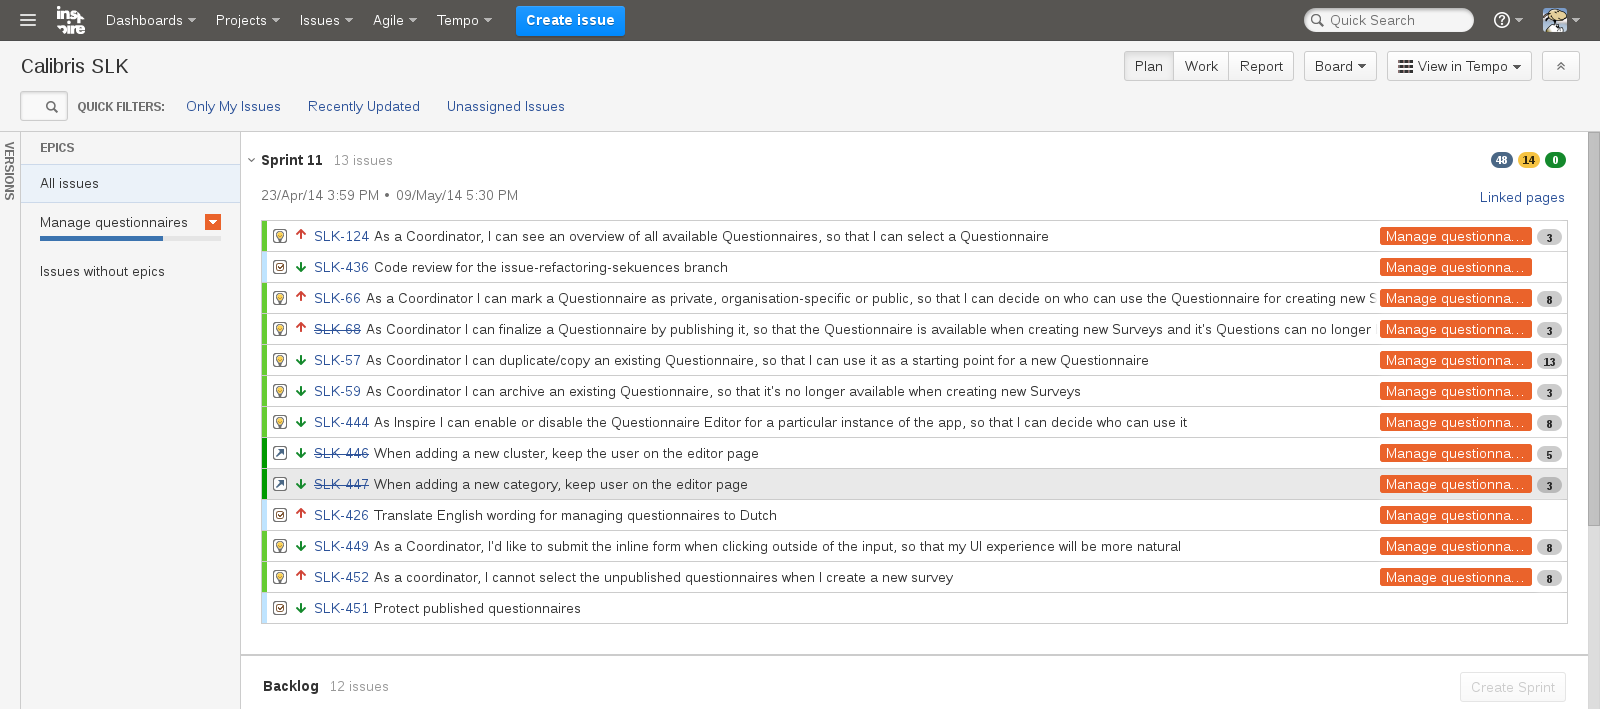
\includegraphics[scale=.30]{img/jira_agile_1.png}
 \caption{Vue des tâches du projet en cours sur le module Agile de Jira}
 \label{fig.jira_agile1}
\end{figure}

\begin{figure}[htp]
\centering
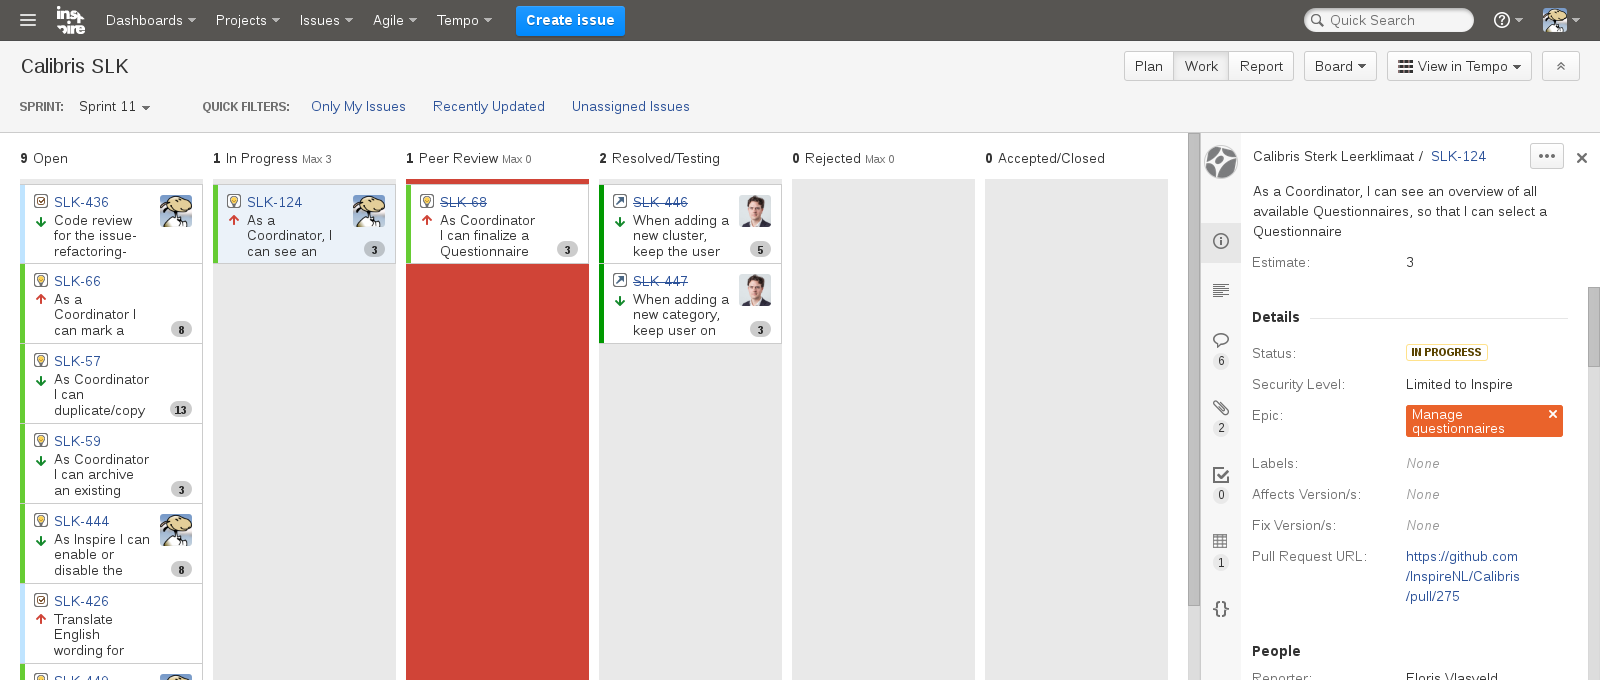
\includegraphics[scale=.30]{img/jira_agile_2.png}
 \caption{Vue du sprint en cours sur le module Agile de Jira}
 \label{fig.jira_agile2}
\end{figure}

Ce module, comme son nom l'indique, permet de gérer de façon efficace l'ensemble des tâches qui sont à effectuer sur les projets en cours. Il se décompose en trois vues :

\begin{description}
  \item[Plan] La vue Plan (voir \cref{fig.jira_agile1}) offre une vue globale de l'ensemble des tâches du sprint actuel mais également des sprints à venir. Les tâches peuvent également être éditées depuis cette interface afin, entre autre, de leurs affecter une difficulté (les nombres de la suite de Fibonacci sont ici utilisés), d'ajouter des commentaires, d'y joindre des documents/images ou d'y affecter une personne de l'équipe.
  \item[Work] Cette vue permet d'organiser les tâches du sprint en cours en suivant les différentes étapes de validation (voir \cref{fig.jira_agile2}). Chacune des tâches se trouve innitialement dans la colonne ``Open'', lors qu'un développeur sera assigné à une tâche (il peut également la choisir lui même) il la déplacera dans la seconde colonne ``In Progress'' et travaillera à sa résolution (en réutilisant la méthodologie précisée dans \cref{sec.git} via la création d'une nouvelle branche sur le dépôt). Lorsque la tâche est finalisée, celle-ci doit encore passer par l'étape ``Peer Review'' afin d'être vérifié par un tiers. Finalement elle sera soit acceptée (cinquième colonne) soit refusée (colonne six), soit renvoyée à l'étape ``Open'' si le second développeur estime que des développements complémentaires sont nécessaires pour la résolution de celle-ci.
  \item[Report] La troisième et dernière vue sert plus au manager. Celle-ci offre des graphiques et statistiques sur le déroulement des différents sprints, la vélocité de l'équipe ou encore la quantité de travail restant à effectuer.
\end{description}

Un système lié à la messagerie interne de l'entreprise (à savoir les comptes mails et de messagerie instantanée) permet à chacun de notifier un, plusieurs ou l'ensemble de ses collègues sur l'évolution ou une difficultée rencontrée sur l'une des tâches.

\subsubsection{Le module Tempo}

En remplacement de l'application Harvest\footnote{\url{http://www.getharvest.com/}} utilisée jusqu'alors, le module Tempo permet à chacun de suivre le temps passé sur chaque tâche. Fortement lié au module précédent, les développeurs et les manageurs peuvent ainsi constater si les estimations faites sur les tâches correspondent au temps utilisé pour leur résolution.

Ce module permet également de savoir quel travail sera facturé au client et de savoir sur quelles tâches le développeur a passé ses quarantes heures de travail hebdomadaires.

\subsection{En bref} 

D'une façon générale, l'ensemble de ces outils sert essentiellement à synchroniser et à garder informé l'ensemble des membres de l'équipe de l'état dans lequel se trouve un projet mais également du travail effectué par leurs collègues.

Quelques autres outils viennent également compléter certains aspects organisationnels tel que Google Calendar\footnote{\url{https://www.google.com/calendar/}} pour la planification des réunions et des évènements internes à l'entreprise ou la messagerie instantanée pour l'envoi rapide de notifications aux différents collaborateurs.

\chapter{Projets}

Au sein de ce chapitre je présenterai les différents projets sur lesquels j'ai pu travailler tout au long du stage, chacun d'entre eux sera composé de trois parties. Je commencerais par faire une présentation générale de l'application et de ses particularités. Puis je reviendrais sur les fonctionnalités qui sont soit à améliorer, soit à développer. J'apporterai par la suite quelques explications détaillées sur des particularités du développement. Finalement je ferais un retour personnel sur les apports de connaissances que j'ai pu avoir tout au long du projet.

\section{Calibris - Gestionnaire de questionnaire}

Calibris est une application développée par Inspire servant à gestion et au remplissage de questionnaires auprès des membres d'une infrastructure.

Suite au développement de cette application un accord est trouvé entre Inspire et le client Innergo\footnote{\url{http://www.innergo.nl/en/index.html}} afin de partager entre les deux entitées la propriété du code-source. Inspire est alors autorisée à continuer le développement sur l'application et de la revendre à d'autres entreprises.

L'idée générale de l'application est de pouvoir importer des questionnaires, les affecter aux différentes structures organisationelles préalablement créées au sein de l'interface et de les transmettres aux collaborateurs de ces mêmes structures. 

L'interface de l'application permet de gérer les structures ainsi que les membres les composants, des rôles pouvant êtres appliqués à certains d'entre eux afin de déléguer certains pouvoirs. 

Les utilisateurs répondants aux questionnaires le font de façon anonyme via la réception d'un lien comportant un numéro unique de session au sein d'un email.

\subsection{Structure d'un questionnaire}

Les questionnaires sont construit suivant trois niveaux. 

\begin{enumerate}
  \item Les catégories qui font office de séparateur permettant de regrouper les questions par thèmes.
  \item Les ``clusters'', sous-catégories, ils permettent d'associer des ensembles de questions traitant des sujets similaires.
  \item Les questions, étants pour le moment de deux types, à réponse ouverte (l'utilisateur a le choix de compléter textuellement sa réponse) ou par une appréciation à cinq niveaux allant de -2 à 2.
\end{enumerate}

Chaque questionnaire possède un titre et une durée moyenne de remplissage arbitrairement définie par le créateur. Les catégories et ``clusters'' possèdent tout deux un nom et sont stockés suivant la même structure dans la base de donnée (un ``cluster'' étant une catégorie ayant comme parent une catégorie).

Les questions possèdent un type, une étiquette (contenant la question en elle même) et un ``cluster'' parent.

Les questionnaires sont intégrés dans l'application via l'importation de tableaux au format CSV (format de tableau simplifié où les cases sont séparées par des virgules) ou Excel.

\begin{figure}[htp]
\centering
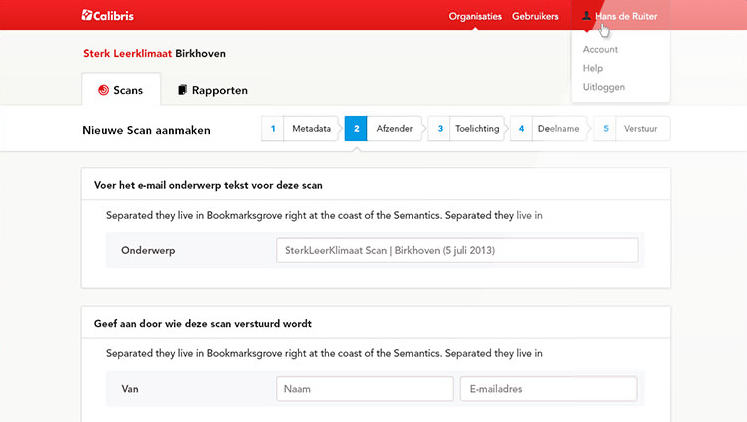
\includegraphics[scale=0.6]{img/calibris1.png}
 \caption{Création d'un nouveau projet de questionnaire sur Calibris}
 \label{fig.calibris1}
\end{figure}

\begin{figure}[htp]
\centering
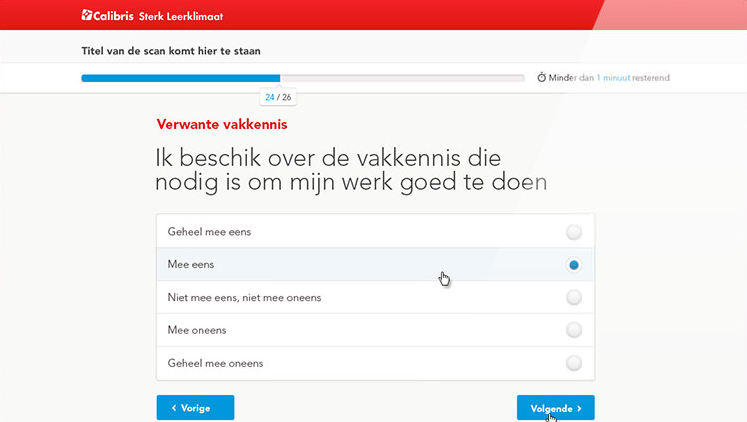
\includegraphics[scale=0.6]{img/calibris2.png}
 \caption{Interface de réponse au questionnaire sur Calibris}
 \label{fig.calibris2}
\end{figure}

\subsection{Travail à effectuer}

Le travail qui m'était demandé devait s'effectuer en deux temps. Inspire ayant acquit une partie des droits d'exploitation de l'application celle-ci souhaite ajouter de nouvelles fonctionnalités qu'elle pourra vendre à de nouveaux clients.

Je devait tout d'abord développer une interface complète permettant de créer, administrer et modifier des questionnaires sans avoir à les importer depuis un fichier externe. Le but général étant donc d'intégrer une interface dynamique permetant la création des différents niveaux (catégories, ``clusters'' et questions) et leurs réorganisations en vue d'une futur publication.

La seconde étape consistant à intégrer cette nouvelle fonctionnalité au reste de l'application via l'interfacage avec les formulaires de gestion des réponses et des droits des utilisateurs.

Pour la réalisation de ce projet je suis épaulée par deux développeurs ayant déjà travaillés plusieurs fois sur le code existant. Ceux-ci m'ont également expliqué en détail de fonctionnement de l'applicaion et des tâches qui m'étaient confiées.

\subsection{Développement}

Dans cette section je reviendrai globalement sur le travail que j'ai eu à effectuer jusqu'alors sur Calibris. Par la suite je détaillerai quelques points technique que j'estime intéressant de préciser.

\subsubsection{Développement général}

Le développement de l'interface d'édition des questionnaire n'a pas réellement causée de grand changement dans la structure même du modèle de données de l'application. L'idée ici étant de pouvoir modifier le contenue des données. Cependant une refactorisation du code source a été nécessaire pour résoudre un problème de structure entre les différents niveaux de l'application.

J'ai donc commencé le développement de façon incrémental via l'implémentation des différentes actions possibles sur chaques types d'éléments du questionnaire. L'idée générale étant de supporter l'ensemble des actions CRUD (create, read, update, delete) pour chacun d'entre eux.

Au fur et à mesure de l'implémentation de ces fonctionnalités j'ai fait valider mon travail par des collègues qui connaissaient déjà particulièrement bien le code existant.

\subsubsection{Utilisation des imbrications d'ensembles}
\label{section.ans}

Comme vu dans le chapitre précédent, un questionnaire possède trois niveaux dont les éléments possèdent chacun un ordre d'apparition bien précis. La structure d'un questionnaire peut donc se représenter par un arbre.

Suite à l'implémentation des première fonctionnalités il est apparu que la structure offerte par défaut pour la liaison des différents modèles de données au sein de Ruby On Rails ne permettait pas d'assurer cet notion d'ordre. De plus la réorganisation de l'ordre des éléments serait source d'une importante activité au niveau de la base de donnée afin de correctement mettre à jour les positions de tout les éléments.

Afin de remédier à ce problème l'équipe a décidée d'utiliser un \textit{gem} exploitant la structure des imbrications d'ensembles\footnote{En informatique, l'imbrication d'ensembles, nested sets en anglais, est une technique pour représenter des données hiérarchisées dans une base de données relationnelle. En substance, elle consiste à attribuer à chaque nœud deux bornes, dite gauche et droite, qui permettent de statuer sur les liens de parentés entre les différents nœuds. Source \url{http://fr.wikipedia.org/wiki/Imbrication_d'ensembles}}

\begin{figure}[htp]
\centering
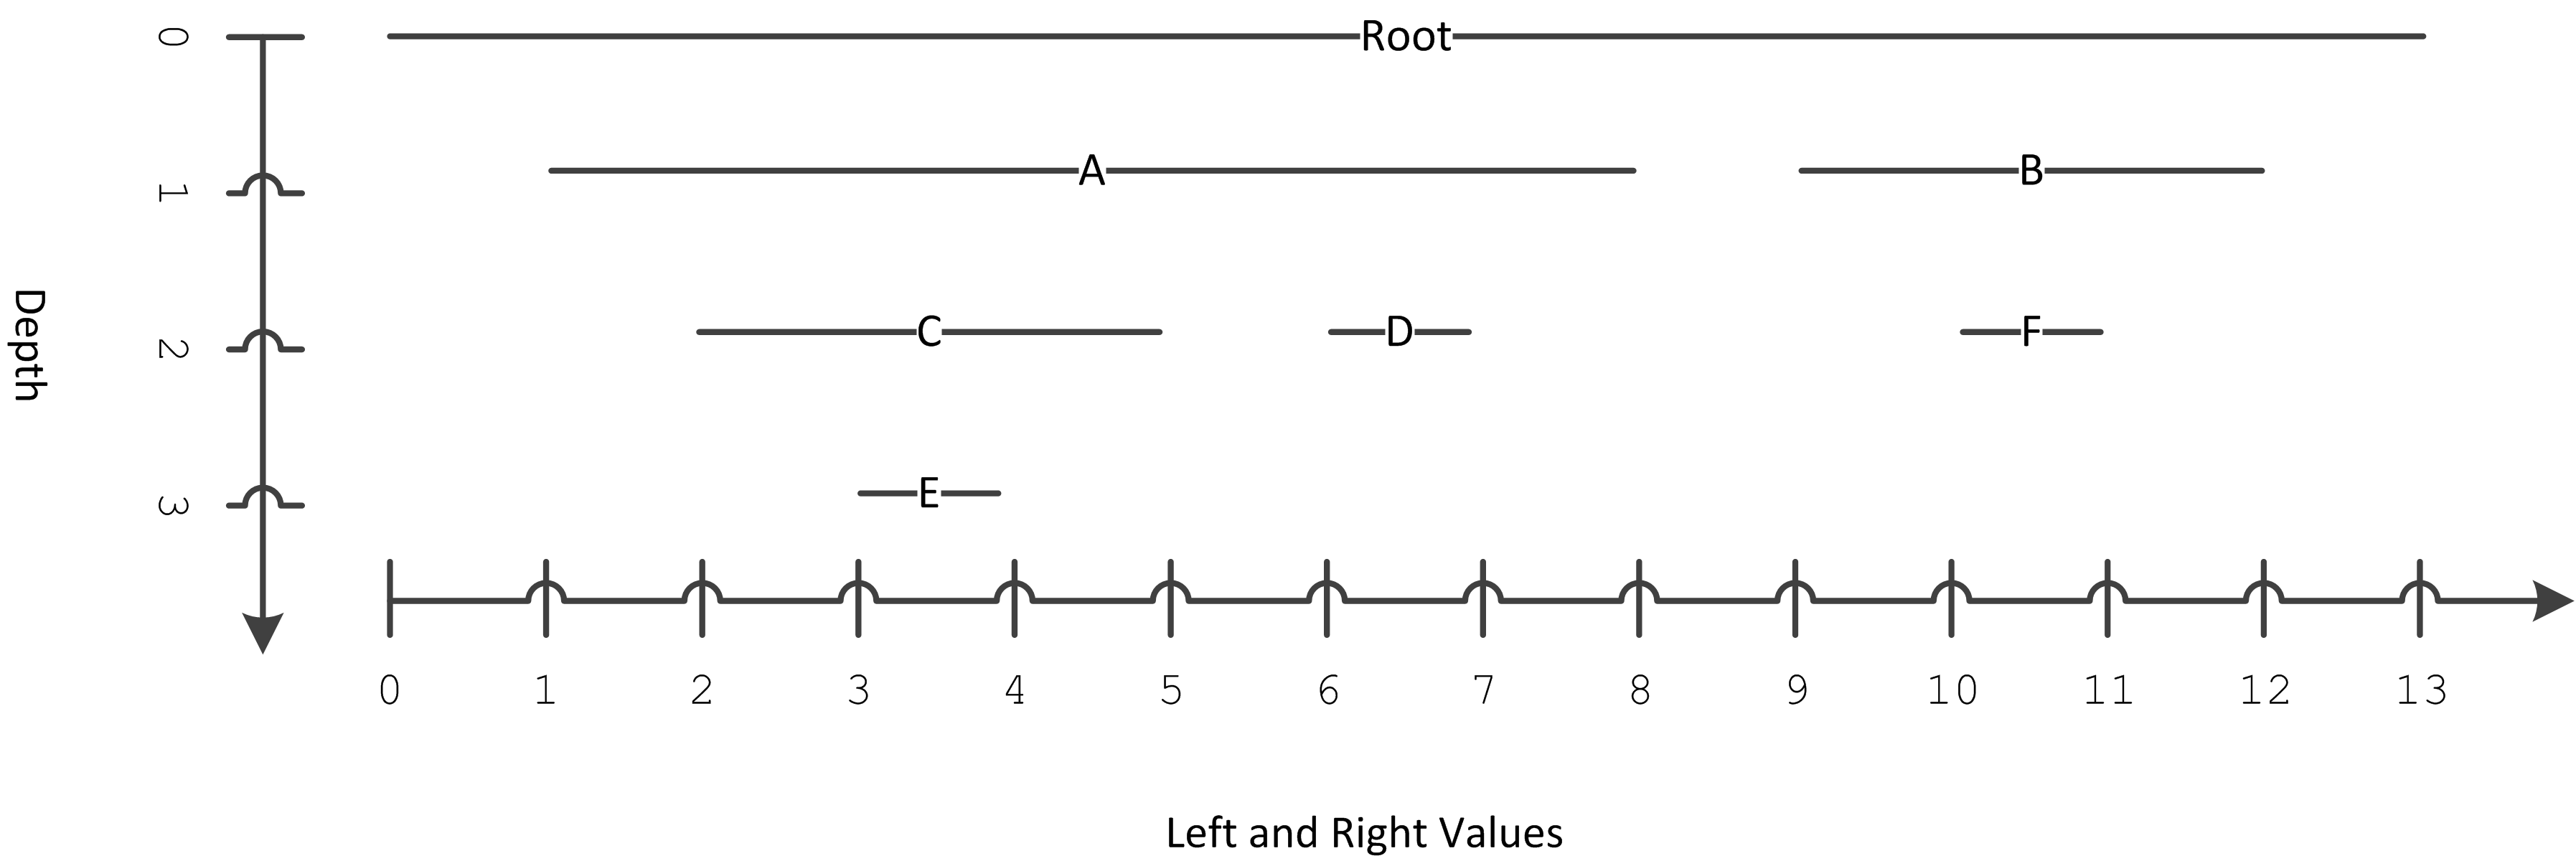
\includegraphics[scale=.12]{img/nested1.png}
\caption{Représentation schématique des nœuds d'un arbre sous forme d'imbrication d'ensembles}
\label{img:nested1}
\end{figure}

L'idée générale peut être schématisée par la \cref{img:nested1}. Chaque nœud de l'arbre possède une valeur ``gauche'' et ``droite'' qui sont respectivement plus grande et plus petite que les valeurs de son propre parent. Ici des nombres entiers sont utilisés afin de faciliter la lecture et l'écriture des valeurs dans une base de donnée SQL mais il est préférable d'utiliser des nombres réels afin d'éviter de mettre à jour de nombreuses valeurs lors du déplacement, de l'ajout ou de la suppresion de nœuds.

Cette structure de données permet également de connaitre de façon très rapide tout les éléments enfants d'un certain nœud via une simple requète d'ordre. Par exemple pour connaitre les enfants de A (soit C, D et E) il suffit de faire une requète similaire à la \cref{fig.nestedsql}.

\begin{figure}[h]
\lstset{language=sql}
\begin{lstlisting}
select * from nodes where lft > 1 and rgt < 8
\end{lstlisting}
 \caption{Exemple de requète SQL sur un arbre ordonné par les ensembles imbriqués}
 \label{fig.nestedsql}
\end{figure}

L'ensemble de ces fonctionnalités sont gérées de façon transparentes par le \textit{gem} AwesomeNestedSet\footnote{\url{https://github.com/collectiveidea/awesome_nested_set}}. Celui-ci permet de convertir un, ou des, modèle(s) d'un projet Ruby On Rails en nœud utilisant cette structure.

\begin{figure}[h]
\lstset{language=ruby}
\begin{lstlisting}
def create
  set_parent_category
  @category = @questionnaire.categories.build(name: name))

  if @category.save
    @category.move_to_child_of(@parent_category) if @parent_category
    flash[:notice] = t('categories.create.success')
  else
    flash[:alert] = t('categories.create.failure')
  end

  redirect_to @questionnaire
end
\end{lstlisting}
 \caption{Exemple de méthode utilisant AwesomeNestedSet}
 \label{fig.nestedrail}
\end{figure}

La \cref{fig.nestedrail} présente une action d'un controlleur de l'application Calibris exploitant la fonctionnalités \texttt{move\_to\_child\_of} offerte par la bibliothèque. Ici l'ensemble des modifications faites à la base de donnée est cachée et sont gérées intelligement par le \textit{gem}.

\subsubsection{Utilisation des \texttt{remote}}

Un autre élément intéressant inhérant à Ruby On Rails et exploité à de multiples reprises dans l'application est la balise \texttt{remote}.

Afin de bien comprendre l'utilité de cette fonctionnalité il faut tou d'abord détailler un peu le fonctionnement du Modèle-Vue-Controlleur au sein de Ruby On Rails.

\paragraph{Le chargement d'une page} passe systématiquement par l'utilisation d'une route unique et prédéfinie dans la configuration de l'application. Nous allons ici prendre l'exemple du chargement de la page \textit{index} du controlleur \textit{QuestionnaireController}.

Cette page possède comme rôle de lister l'ensemble des questionnaires actuellement présents dans la base de donnée de l'application. Elle est accessible par le chemin \texttt{questionnaires\_path}, chemin qui retourne une URL correspondant à l'adresse exacte de la page (dans notre cas il s'agit de \url{http://localhost:3000/questionnaires}).

Lorsque nous allons visiter cette URL (via un lien interne à l'application ou en rentrant directement l'adresse dans la barre du navigateur), le framework va alors tenter de charger plusieurs éléments.

\begin{enumerate}
  \item Il va tout d'abord interroger le Controlleur correspondant à l'URL interrogée, dans notre cas il s'agit de QuestionnaireController.
  \item Puis il va cherche l'action spécifique à exécuter au sein du Controlleur. Si aucune action n'est spécifiée (ce qui est ici le cas puisque rien n'a été précisé à la fin de l'URL) c'est l'action \texttt{index} qui est exécutée.
  \item Le framework va alors exécuter la méthode \texttt{index} du controlleur, celle-ci s'occupera du rendu de la page \texttt{index.html}, laquelle sera renvoyée au navigateur.
\end{enumerate}

\paragraph{Dans certains cas} nous ne souhaitons pas générer une page XHTML classique mais plutôt exécuter du code Javascript afin d'effectuer une transformation particulière sur la page courante. Dans ce cas précis nous ne voulons pas appeler l'action (qui, rappelons le correspond à une méthode du Controlleur) via le chargement d'une page mais plutôt de façon asynchrone via une requète Ajax\footnote{L'architecture informatique Ajax (acronyme d'Asynchronous JavaScript and XML) permet de construire des applications Web et des sites web dynamiques interactifs sur le poste client en se servant de différentes technologies ajoutées aux navigateurs web entre 1995 et 2005. \url{http://fr.wikipedia.org/wiki/Asynchronous_JavaScript_and_XML}}. 

\paragraph{L'ajout d'un lien} dans une vue Rails se fait d'une façon similaire au code de la \cref{fig.link}. Ici nous appelons la fonction \texttt{link\_to} qui génèrera une balise \texttt{a} possédant un titre et une classe. La valeur du lien (correspondant au contenu de l'attribut \texttt{href}) est le résultat de la fonction \texttt{questionnaires\_path}.

Ce code génèrera un lien XHTML similaire à la \cref{fig.link2}.

\begin{figure}[h]
\lstset{language=ruby}
\begin{lstlisting}
link_to questionnaires_path, 
  title: t('questionnaires.title'), 
  class: 'questionnaire-edit'
\end{lstlisting}
 \caption{Extrait d'une vue s'occupant de la génération d'un lien}
 \label{fig.link}
\end{figure}

\begin{figure}[h]
\lstset{language=xml}
\begin{lstlisting}
<a href="http://localhost:3000/questionnaires/" 
   title="Les Questionnaires" 
   class="questionnaire-edit"/>
\end{lstlisting}
 \caption{Exemple de code généré à partir de la \cref{fig.link}}
 \label{fig.link2}
\end{figure}

\paragraph{L'ajout du paramètre \texttt{remote}} à la fonction \texttt{link\_to} va permettre de changer radicalement le comportement du lien. En effet, lors du clic sur celui-ci, le navigateur ne va pas se diriger vers la nouvelle page mais plutôt générer une requête Ajax qui ira interroger l'action en question dans la classe QuestionControlleur. Le résultat attendu n'est donc pas une page XHTML mais plutôt du code Javascript ou un pouvant être traité par le navigateur lors de la génération de la réponse par le serveur.

L'ensemble de ce mécanisme est automatiquement généré par le framework Ruby On Rails dès le simple ajout de cet attribut.

Lors de mon développement j'ai donc utilisé à mainte reprises ce mécanisme afin de pouvoir remplacer des éléments du contenu des questionnaires pour les remplacer par un formulaire d'édition. De cette façon l'utilisateur n'a qu'à cliquer directement sur l'élément pour que celui-ci soit replacé par une balise d'édition permettant la modification dynamique de la valeur du champ sans rechargement de page.  

\subsubsection{Utilisation de jQuery Sortable}

La bibliothèque jQuery Sortable\footnote{\url{http://jqueryui.com/sortable/}} est une extension à la bibliothèque jQuery permettant la réorganisation des éléments d'une page XHTML via le déplacement sous forme de ``drag \& drop'' des blocs en question.

Après avoir correctement chargé les deux librairies (jQuery et jQuery Sortable) un petit peu de Javascript est à rédiger afin de faire le lien avec les éléments que nous souhaitons animer.

Le but ici étant de pouvoir réorganiser les différents éléments du questionnaire en cours d'édition (les catégories, clusters et questions) puis de sauvegarder ces mêmes modifications sur le serveur.

La déclaration d'une liste en tant qu'éléments ``sortables'' est assez simple et le comportement peut être facilement personnalisé. Comme la \cref{fig.sort1} le montre l'idée est simplement de rechercher un élément appelé ``parent'' qui servira de conteneur aux déplacement des blocs. Nous déclarons ensuite l'ensemble des enfants qui pourront être déplacés via l'utilisation d'un second sélecteur (ici définit par la clef \texttt{items}).

La clef \texttt{update} permet d'appeler une fonction Javascript particulière lorsque le déplacement est terminé (pour, par exemple, permettre de sauvegarder les modifications sur le serveur). Finalement, le mot clef \texttt{handle} permet de définir une zone sur chaque élément déplacable qui servira de poignée pour faciliter leurs réorganisation.

\begin{figure}[h]
%\lstset{language=js}
\begin{lstlisting}
$(".container.total_scores.questionnaires.sortable").sortable
    items: ".category_sortable"
    update: sortCategory
    handle: "th.score.grip"
\end{lstlisting}
 \caption{Déclaration d'une liste d'éléments ``sortables''}
 \label{fig.sort1}
\end{figure}

Dans mon cas il fallait que j'envois la nouvelle position de l'élément changé afin de mettre à jour l'arbre déclaré dans la base de donnée. Pour cela, chaque élément affiché possède un identifiant unique qui se trouve être celui issue de la base de donnée. Ainsi lors de la mise à jour je n'avait qu'à récupérer l'idéntifiant de l'élément parent, de l'élément à gauche et, si possible de l'élément à droite (dans le cas particulier ou l'élément serait déplacé en tout début de ``sous-liste'') puis de mettre à jour correctement mon modèle de donnée à partir de ces informations.

Le parent est ici également envoyé car nous avons autorisé le déplacement d'un élément d'un sous-branche à une autre.

\begin{figure}[h]
%\lstset{language=js}
\begin{lstlisting}
sortQuestion = (event, ui) ->
  items = $(this)
  params = {}
  if ui.item.context.className is "question_sortable"
    context = ui.item.context
    params["parent"] = context.parentNode.parentNode.parentNode.parentNode.id
    if context.previousElementSibling and context.previousElementSibling.id isnt ""
      params["previous"] = context.previousElementSibling.id
    if context.nextElementSibling and context.nextElementSibling.id isnt ""
      params["next"] = context.nextElementSibling.id 
  $.ajax
    url: ui.item.data("sort-url")
    type: "post"
    data: params
    dataType: "script"
    complete: (request) ->
      items.effect "highlight"
      return
\end{lstlisting}
 \caption{Mise à jour des informations lors du déplacement d'une question}
 \label{fig.sort2}
\end{figure}

Dans l'exemple de la \cref{fig.sort2} nous pouvons observer deux étapes. Tout d'abord la fonction va tenter de récupérer toutes les informations nécessaires à la bonne compréhension de la nouvelle proposition de l'élément en récupérant les identifiants des éléments à gauche et à droite (respectivement récupérés grâce à l'utilisation de la primitive DOM\footnote{Le Document Object Model (ou DOM) est un standard du W3C qui décrit une interface indépendante de tout langage de programmation et de toute plate-forme, permettant à des programmes informatiques et à des scripts d'accéder ou de mettre à jour le contenu, la structure ou le style de documents XML et HTML1. Le document peut ensuite être traité et les résultats de ces traitements peuvent être réincorporés dans le document tel qu'il sera présenté. Source \url{http://fr.wikipedia.org/wiki/Document_Object_Model}} \texttt{previousElementSibiling} et \texttt{nextElementSibling} et le parent.

Par la suite nous envoyons une simple requête Ajax vers le serveur avec ces informations et nous affichons un petit effet de surlignage (``highlight'') afin de confirmer la bonne prise en compte des informations.

La méthode \texttt{sort} Ruby On Rails présentée \cref{fig.sort3} permet de comprendre facilement comment les informations fraichement récupérées du navigateur vont servir à mettre à jour la base de donnée. 

Ici nous réutilisons des primitives du \textit{gem} AwesomeNestedSet présenté en \cref{section.aws}. Tout d'abord nous affection notre élément déplacé (ici une question) à son nouveau parent avant de le déplacer à gauche, ou a droite d'un de ses éléments frères suivant sa position dans la sous branche.

Cet méthode peut ici être facilement testée en vérifiant les positions de chaques élément après un déplacement dont le résultat est connu.

\begin{figure}[h]
\lstset{language=ruby}
\begin{lstlisting}
def sort
  @category = Category.find(params[:parent])

  @question.category = @category
  @question.save

  if params[:previous]
      @question.move_to_right_of params[:previous].to_i
  elsif params[:next]
      @question.move_to_left_of params[:next].to_i
  end

  render nothing: true
end
\end{lstlisting}
 \caption{Mise à jour des informations lors du déplacement d'une question}
 \label{fig.sort3}
\end{figure}

\subsubsection{Backend en full Ruby On Rails}


- Backend en full rail
- Structure de données

\listoffigures

\printglossaries

\newpage
\vspace*{\stretch{1}}
\section*{Licence}
\begin{center}
Ce présent document est livré avec ses sources sous licence\\
\ccby Creative Commons Attribution 3.0 Unported Licence.
\end{center}

\paragraph*{Vous êtes libre de}

\begin{itemize}
\item \textbf{partager} — reproduire, distribuer et communiquer l'\oe uvre
\item \textbf{remixer} — modifier l'\oe uvre
\end{itemize}

\paragraph*{Selon les conditions suivantes}
Paternité — Vous devez attribuer l'\oe uvre de la manière indiquée par l'auteur de l'\oe uvre ou le titulaire des droits (mais pas d'une manière qui suggérerait qu'ils vous soutiennent ou approuvent votre utilisation de l'\oe uvre). 

\paragraph*{La version intégrale du contrat est disponible à cette adresse}

\begin{center}
\textit{http://creativecommons.org/licenses/by/3.0/}
\end{center}
\vspace*{\stretch{1}}

\end{document}
